\section{Search} \label{sec:Search}
%\subsection{Realizing Text and Formula search for \oeis}

{\mws} (\mwss) \cite{KohPro:man13} is an open-source, open-format, content-oriented search
engine for mathematical expressions. We refer to \cite{KohPro:man13} for details.

To realize the search instance in \mwss we need to provide two things:
\begin{compactenum}
 \item A \emph{harvest} of \mathml-enriched \html files that the search system can resolve queries against.
 The content-\mathml from the files will be used to resolve the formula part of the query while the rest of the \html
will be used for the text part. The harvest additionally requires a configuration file
that defines the location in the \html files of \mwss-relevant metadata such as the title, author or URL of the
original
article. This, together with the \html itself is used when presenting the query results.
 \item A \emph{formula converter} that converts a text-based formula format into \mathml. This will be used so that
 we can input formulas for searching in a text format (in our case \oeis-inspired ASCII math syntax) rather than
 writing
 \mathml directly.
\end{compactenum}

\begin{figure}
\centering
 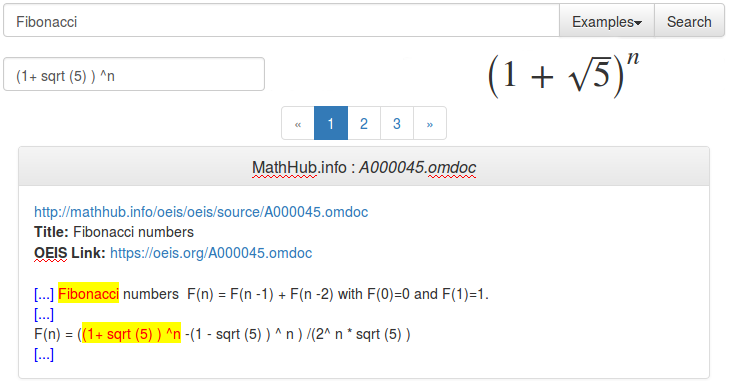
\includegraphics[width=15cm]{search.png}
 \caption{Text and Formula Search for \oeis}\label{fig:search}
\end{figure}

To produce the harvest of the \oeis library for \mwss we export the \html from the content
imported into \mmt. We reuse the \mmt presentation framework and only enhance it with
\oeis-specific technicalities such as sequence name or \oeis link. For the formula
converter we use the same parser used for \oeis formulas and described above, except
extended with one grammar rule for \mwss \emph{query variables}. We then forward the
resulting formula in \mmt to produce the presentation (\mathml) and return it to the \mwss
frontend.  The web-server infrastructure, needed to communicate with \mwss, is provided by
\mmt and we just extend it. Figure \ref{fig:search} shows (a part of) the current
interface answering a query about Fibonacci numbers. The search system is available at
\url{http://oeissearch.mathweb.org}.



%%% Local Variables:
%%% mode: latex
%%% TeX-master: "../report"
%%% End:
